%%%%%%%%%%% Single Column %%%%%%%%%%%%%%%%%
\documentclass[review, 1p, number, sort&compress,table]{elsarticle}
%%%%%%%%%% Double Column %%%%%%%%%%%%%%%%%%%
%\documentclass[preprint, 3p, twocolumn, number, sort&compress,table]{elsarticle}
%%%%%%%%%%%%%%%%%%%%%%%%%%%%%%%%%%%%%%%%%%%%%   
\journal{Acta Materialia}

\usepackage{styles/mainStyles}   % Set for for extra stylings
\usepackage{indentfirst}
\usepackage{epstopdf}
\usepackage{CJK}  
\usepackage{amsmath}

% hyperlinking is set to color blue.
% \autoref is currently set to cross references figures as 'Fig. 1', and equations as 'Eq.1'. 
%This can be changed
%%%%%%%%%%%%%%%%%%%%%%%%%%%%%%%%%%%%%%%%%%%%
% --------------Custom Commands-------------%
%for more info go to ``styles\mainStyles.sty''
% \textgreek - enables greek letters outside of math mode (ie. \textalpha, \textgamma)
% \celcius   - for degrees C  
% \etal      - produces italic ``et al.''
% \um        - for micrometers
% \mc{23}{6}  - produces ``M23C6'' carbides. Can change values.
% Various Differential equation --- look at documentation for mor info 
%%%%%%%%%%%%%%%%%%%%%%%%%%%%%%%%%%%%%%%%%%%%
\begin{document}
	\begin{frontmatter}
		\title{Scaling Analysis of a Moving Guassion Heat Source in Steady State in a Semi-Infinite Solid}
		
		\author[UoA]{X.~Y.~Jimmy\corref{cor1}}
		\ead{jimmy@ualberta.ca}
		%\ifpdf
		%	\ead{jimmy@ualberta.ca}
			%\ead{\href{mailto:jimmy@ualberta.ca}{jimmy@ualberta.ca}}
		%\else
		%	\ead{jimmy@ualberta.ca}
		%\fi
		
		\author[UoA]{P.~F.~Mendez}
		\ead{pmendez@ualberta.ca}
		%\ifpdf
		%	\ead{pmendez@ualberta.ca}
		%	%\ead{\href{mailto:pmendez@ualberta.ca}{pmendez@ualberta.ca}}
		%\else
		%	\ead{pmendez@ualberta.ca}
		%\fi
		
		\cortext[cor1]{Corresponding author. Tel: +1-780-XXX-XXXX}
		
		\address[UoA]{Department of Chemical and Materials Engineering, University of Alberta, Edmonton, Alberta,T6G 2V4, Canada}
	
		\begin{abstract}
			Abstract goes here
		\end{abstract}
		
		\begin{keyword}
			keyword1 \sep keyword2 \sep keyword3 \sep keyword4
		\end{keyword}

	\end{frontmatter}
	
	%%%%%%%%%%%%%%%%%%%%%%%%%%%%%%%%%%%%%%%%%%%%%%%%%%
%%%             INTRODUCTION SECTION              %%%%
%%%%%%%%%%%%%%%%%%%%%%%%%%%%%%%%%%%%%%%%%%%%%%%%%%	

	\section{Introduction}
		\indent 
		Our research focuses on developing simplified formulas with high accuracy that will substitute complex numerical calculations. 
		      
	\section{Governing Equation}\label{sec:governing}
		\begin{equation}  \label{eq:original}
		T^*=\frac{1}{\sqrt{2\pi}}\int_{0}^{\infty}{d\tau}\frac{\tau^{-\frac{1}{2}}}{\tau+\sigma^{*2}}e^{-\frac{x^{*2}+2\tau^*x^{*}+\tau^{*2}+y^{*2}}{2\tau+2\sigma^{*2}}-\frac{z^{*2}}{2\tau}}
		\end{equation}
		\autoref{eq:original} has some disadvantages. Firstly, it is a improper integral and the up limit is infinity which makes the calculation more difficult. Secondly, the integrand has two peaks. One locates at $\tau=0$, and the other moves and is hard to determine, which may results in the omitting of second peak in integral.  \\
		Use variable substitution method $t=\arctan{\frac{\sqrt{\tau}}{\sigma}}$,and do not consider the depth of  pool, which means $z^*=0$.
		\begin{equation} \label{eq:gover}
		T^{*}=\frac{2}{\sqrt{2\pi}\sigma^*}\int_{0}^{\frac{\pi}{2}} e^{-\frac{1}{2}\left[\sigma^{*2}\left(\cos^2{t}+\frac{1}{\cos^2{t}}-2 \right)+\frac{\cos^2{t}\left(x^{*2}+y^{*2}\right) }{\sigma^{*2}}+2x^{*}\left( 1-\cos^2{t} \right)          \right] }dt
		\end{equation}
		\autoref{eq:gover} avoids the disadvantages of \autoref{eq:original}. The integral  is bounded. The integrand has one peak located  at $t=\arccos{\{\sigma^{*}[(\sigma^{*2}-x^{*})^2+y^{*2}]}\}$ . However, \autoref{eq:gover} can't be applied to the point-source condition.   \\ 
		
	\section{the highest $T^{*}$ corresponding to $\sigma^{*}$}\label{sec:2}	
	To calculating the highest $T^{*}$ corresponding to $\sigma^{*}$, $y^{*}$ should be set as $0$.\\
	\subsection{$\sigma\rightarrow{0}$}
	According the numerical calculation, $x^{*}$ should be much smaller than $\sigma^{*}$,so $|\frac{x^{*}}{\sigma^{*}}|\sim 0$ . \autoref{eq:gover} can be simplified as:	
		\begin{eqnarray} \label{eq:TvS.0}
				\nonumber 
				T^{*}_{m\uppercase\expandafter{\romannumeral1}} =\frac{2}{\sqrt{2\pi}\sigma^*}\int_{0}^{\frac{\pi}{2}} e^{-\frac{1}{2}\left[\sigma^{*2}\left(\cos^2{t}+\frac{1}{\cos^2{t}}-2 \right)+\frac{\cos^2{t} \; x^{*2}}{\sigma^{*2}}+2x^{*}\left( 1-\cos^2{t} \right)\right] }dt
				\\  \nonumber 
				\approx\frac{2}{\sqrt{2\pi}\sigma^*}\int_{0}^{\frac{\pi}{2}} e^{-\frac{1}{2}\sigma^{*2}\left(\cos^2{t}+\frac{1}{\cos^2{t}}-2 \right) }dt
				\\ 
				\approx \frac{2}{\sqrt{2\pi}\sigma^*}\frac{\pi}{2} = \sqrt{\frac{\pi}{2}}    \; \sigma^{*-1} 
		\end{eqnarray}
	\subsection{$\sigma\rightarrow{\infty}$}
	When $\sigma$ tends to infinity, the peak locates at $0$, and the integrand decreases sharply. 	
		\begin{eqnarray} \label{eq:TvS.inf.1}
		\nonumber 
		T^{*}_{m\uppercase\expandafter{\romannumeral2}} =\frac{2}{\sqrt{2\pi}\sigma^*}\int_{0}^{\frac{\pi}{2}} e^{-\frac{1}{2}\left[\sigma^{*2}\left(\cos^2{t}+\frac{1}{\cos^2{t}}-2 \right)+\frac{\cos^2{t} \; x^{*2}}{\sigma^{*2}}+2x^{*}\left( 1-\cos^2{t} \right)\right] }dt
		\\ \nonumber
		\approx  \frac{2}{\sqrt{2\pi}\sigma^*}\int_{0}^{\delta} e^{-\frac{1}{2}\left[\sigma^{*2}\left(\cos^2{t}+\frac{1}{\cos^2{t}}-2 \right)+\frac{\cos^2{t} \; x^{*2} }{\sigma^{*2}}+2x^{*}\left( 1-\cos^2{t} \right)\right] }dt
		\\ \nonumber
		\approx  \frac{2}{\sqrt{2\pi}\sigma^*}\int_{0}^{\delta} e^{-\frac{1}{2}\left[\sigma^{*2}\;t^4+\frac{(1-t^2)x^{*2} }{\sigma^{*2}}+2x^{*}t^2 \right] }dt
		\\ \nonumber		
		= \frac{2}{\sqrt{2\pi}\sigma^*}\int_{0}^{\delta} e^{-\frac{1}{2}\left[\sigma^{*2}\;t^4+(2x^{*}-\frac{x^{*2}}{\sigma^{*2}})t^2 +\frac{x^{*2}}{\sigma^{*2}}\right] }dt
		\\ \nonumber
		\approx \frac{2}{\sqrt{2\pi}\sigma^*}\int_{0}^{\delta} e^{-\frac{1}{2}\left[\sigma^{*2}\;t^4+2x^{*}t^2 +\frac{x^{*2}}{\sigma^{*2}}\right] }dt
		\\ \nonumber
		\approx \frac{2}{\sqrt{2\pi}\sigma^*}\int_{0}^{\delta} e^{-\frac{1}{2}\left(\sigma^{*}t^2+\frac{x^{*}}{\sigma^{*}}\right)^2 }dt
       \\ 
       	\approx \frac{2}{\sqrt{2\pi}\sigma^*}\int_{0}^{\frac{\pi}{2}} e^{-\frac{1}{2}\left(\sigma^{*}t^2+\frac{x^{*}}{\sigma^{*}}\right)^2 }dt
		\end{eqnarray}
	Where $\delta$ is infinitesimal, and $x^{*} \sim \sigma^{*} \gg 1$.
	\\
	Use numerical method to find the maximum value of \autoref{eq:TvS.inf.1} with changes of $x^{*}$. When $x^{*}=-0.7650 \;\sigma^{*}$, $T^{*}$ reaches maximum value.
		\begin{equation} \label{eq:TvS.inf}
			T^{*}_{m\uppercase\expandafter{\romannumeral2}}= \frac{2.5596}{\sqrt{2\pi}} \; \sigma^{*-1.5}
		\end{equation}
	\subsection{blending}
	Use \autoref{eq:TvS.0} and  \autoref{eq:TvS.inf} to obtaining the blending equation for all $\sigma$.
	\begin{equation} \label{eq:TvS}
		T^*_m=\left[ \left( \sqrt{\frac{\pi}{2}}    \; \sigma^{*-1}\right)^n+ \left(\frac{2.5596}{\sqrt{2\pi}} \; \sigma^{*-1.5}\right)^n\right]^{\frac{1}{n}}
	\end{equation}
	Where $n=-1.9464$, and the maximum error reaches $0.1901\%$. \\
		\begin{figure*}[ht!]
			\begin{center}
				\subfloat[correspondence between $T^*_m$ and $\sigma^{*}$]{\label{fig:TvS}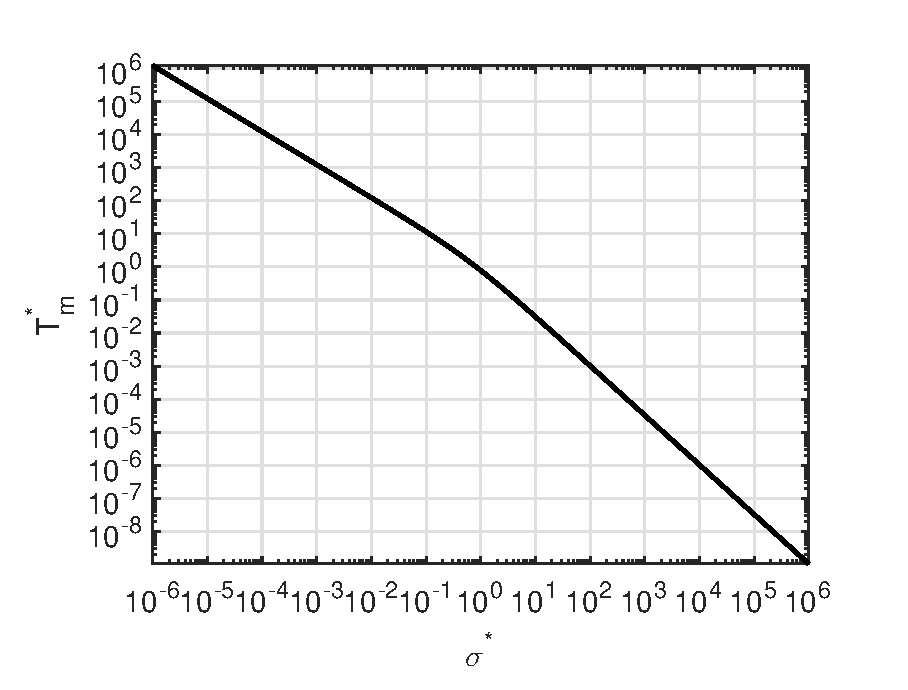
\includegraphics[width=2.2in]{TvS}}
		 		\subfloat[relative error changes with $\sigma^{*}$ when $n=-1.9464 $]{\label{fig:EvS}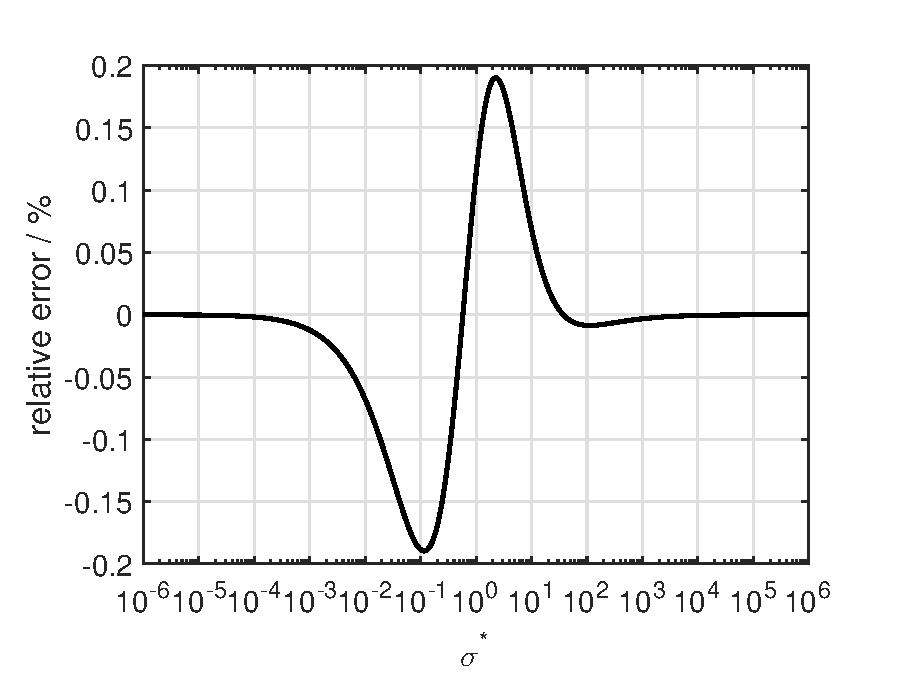
\includegraphics[width=2.2in]{EvS}}
				\subfloat[maximum error changes with n around $-1.9464$]{\label{fig:Evn@TvS}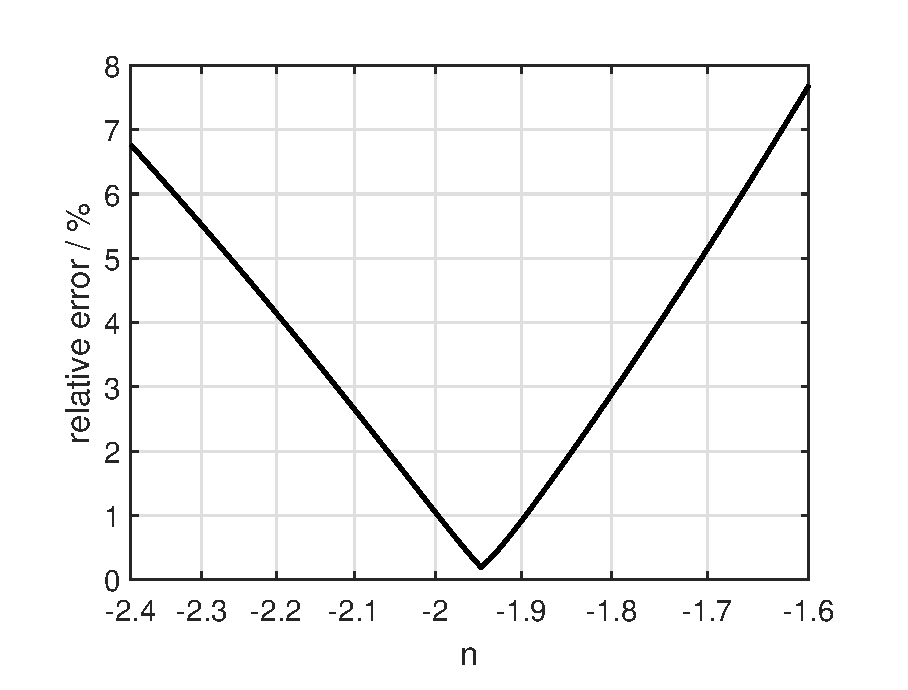
\includegraphics[width=2.2in]{Evn@TvS}}
			\end{center}
			\caption{Results of the blending between $T^*_m$ and $\sigma^{*}$  }
			\label{fig:A.TvS}
		\end{figure*}

	\autoref{eq:TvS} reveals the one-to-one correspondence between $\sigma^*$ and $T^{*}$. For any melting point $T^*$, there is a certain $\sigma^{*}$, below which the base substance can't melt, and vice versa. So, \autoref{eq:TvS.0} and \autoref{eq:TvS.inf} can be rewritten as:
	\begin{equation}  \label{eq:SvT.0}
		\sigma^{*}_{m\uppercase\expandafter{\romannumeral1}}=\sqrt{\frac{\pi}{2}}Ry^{*}
	\end{equation}
	Where $Ry^{*}=\frac{1}{T^{*}}$.  \\
	\begin{equation}  \label{eq:SvT.inf}
		\sigma^{*}_{m\uppercase\expandafter{\romannumeral2}}=1.0140 \; Ry^{*\frac{2}{3}}
	\end{equation}
	\begin{equation}  \label{eq:SvT}
	\sigma^{*}_{m}=\left[ \left( 1.0140 \; Ry^{*\frac{2}{3}}\right)^n+ \left( \sqrt{\frac{\pi}{2}}Ry^{*}\right)^n\right]^\frac{1}{n}
	\end{equation}
	Where $n=-2.3975$, and the maximum error reaches minimum, $1.39\%$.
			\begin{figure*}[ht!]
				\begin{center}
					\subfloat[correspondence between $\sigma^*_m$ and $Ry^{*}$]{\label{fig:SvR}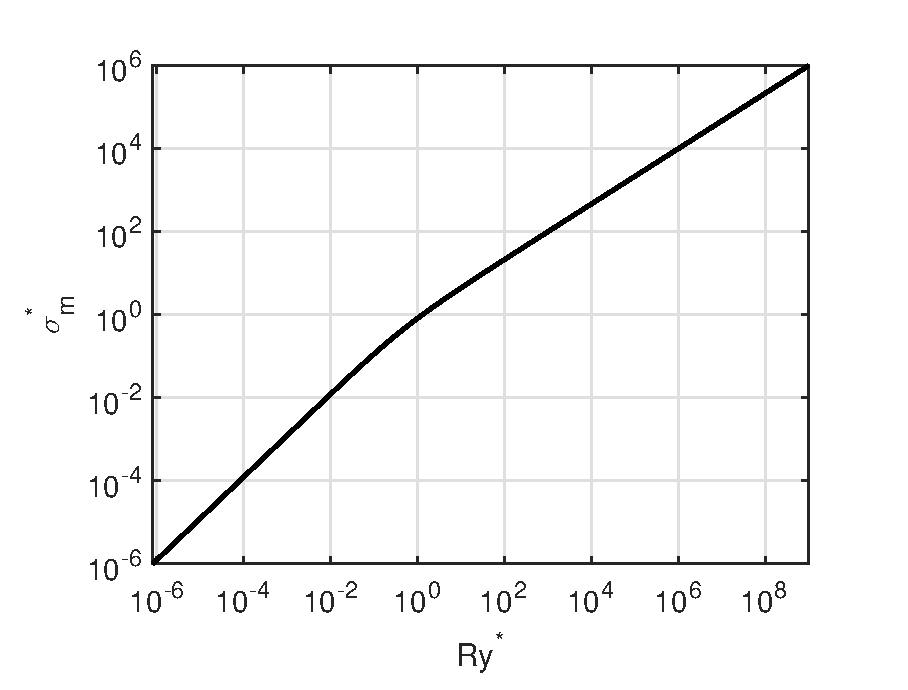
\includegraphics[width=2.2in]{SvR}}
					\subfloat[relative error changes with $Ry^{*}$ when $n=-2.3975 $]{\label{fig:EvR.SvR}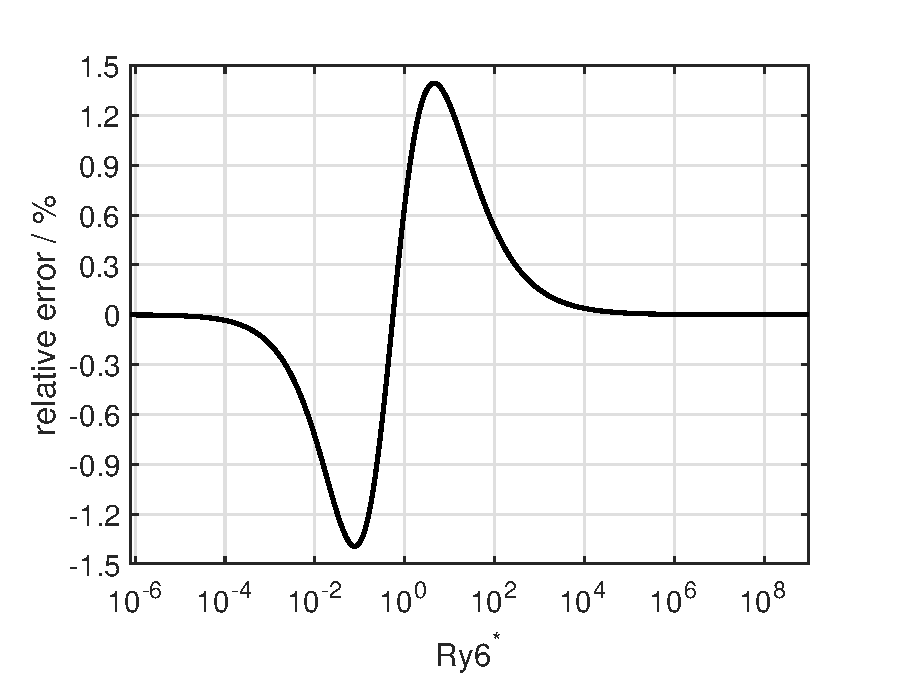
\includegraphics[width=2.2in]{EvR@SvR}}
					\subfloat[maximum error changes with n around $-2.3975$]{\label{fig:Evn.SvR}\includegraphics[width=2.2in]{Evn@SvR}}
				\end{center}
				\caption{Results of the blending between $\sigma^*_m$ and $Ry^{*}$  }
				\label{fig:A.SvR}
			\end{figure*}
			\\
			
	\section{$\sigma\rightarrow{\sigma_m}$}
	When $\sigma^{*}$ tends to $\sigma^{*}_m$, the welding pool vanishes, and should be axisymmetric, which means the maximum width point locates above the maximum temperature point, i.e. $x_{m,\mbox{corresponding to maximum width point}}=x_{m,\mbox{corresponding to maximum temperature point}}$.
	\subsection{$\sigma\rightarrow{0}$}
		\begin{eqnarray}
		\nonumber
			T^{*}_{\uppercase\expandafter{\romannumeral1};x_0,y}=\frac{2}{\sqrt{2\pi}\sigma^*}\int_{0}^{\frac{\pi}{2}} e^{-\frac{1}{2}\left[\sigma^{*2}\left(\cos^2{t}+\frac{1}{\cos^2{t}}-2 \right)+\frac{\cos^2{t}\left(x^{*2}_0+y^{*2}\right) }{\sigma^{*2}}+2x^{*}_0\left( 1-\cos^2{t} \right)\right] }dt
			\\ \nonumber
			=\frac{2}{\sqrt{2\pi}\sigma^*}\int_{0}^{\frac{\pi}{2}} e^{-\frac{1}{2}\left[\sigma^{*2}\left(\cos^2{t}+\frac{1}{\cos^2{t}}-2 \right)+\frac{\cos^2{t}\;x^{*2}_0 }{\sigma^{*2}}+2x^{*}_0\left( 1-\cos^2{t} \right)\right]} \cdot e^{-\frac{\cos^2{t}y^{*2}}{2\sigma^{*2}}}dt
			\\ \nonumber	
			\approx \frac{2}{\sqrt{2\pi}\sigma^*}\int_{0}^{\frac{\pi}{2}} 1 \cdot e^{-\frac{\cos^2{t} \; y^{*2}}{2\sigma^{*2}}}dt
			 \\ \nonumber
			=\frac{2}{\pi}T^{*}_{\uppercase\expandafter{\romannumeral1};x_0,y=0} \cdot \int_{0}^{\frac{\pi}{2}} e^{-\frac{\cos^2{t} \; y^{*2}}{2\sigma^{*2}}}dt
			\\ \nonumber
			\approx \frac{2}{\pi}T^{*}_{\uppercase\expandafter{\romannumeral1};x_0,y=0} \cdot \int_{0}^{\frac{\pi}{2}} 1-\frac{\cos^2{t} \; y^{*2}}{2\sigma^{*2}}dt \quad \quad  \mbox{as $y^{*}\ll \sigma^{*}$}
			\\  \nonumber
			=	 T^{*}_{\uppercase\expandafter{\romannumeral1};x_0,y=0}\cdot
			 \frac{2}{\pi}\left(\frac{\pi}{2}-\frac{y^{*2}\pi}{8\sigma^{*2}}\right)
			\\ \nonumber
			=	 T^{*}_{\uppercase\expandafter{\romannumeral1};x_0,y=0}\cdot
			\left(1-\frac{y^{*2}}{4\sigma^{*2}}\right)
			\\ \nonumber
			=	 T^{*}_{\uppercase\expandafter{\romannumeral1};x_0,y=0}\cdot
			\left(1-\frac{y^{*2}}{4\sigma^{*2}}\right)
			\\ 
			=	 T^{*}_{\uppercase\expandafter{\romannumeral1};x_0,y=0}\cdot
			e^{-\frac{y^{*2}}{4\sigma^{*2}}} \label{eq:near field.0}
		\end{eqnarray}
	Where $x_0^{*}=0$, $y^{*}\ll \sigma^{*}$.  \\
	According to \autoref{eq:near field.0}, 
	\begin{equation} \label{eq:Sm.0}
		y_{m\uppercase\expandafter{\romannumeral1}}^{*} = 2\sigma^{*}\sqrt{\ln{\frac{T^{*}(\sigma^{*})}{T^{*}}}}=2\sigma^{*}\sqrt{\ln{\frac{Ry^{*}}{Ry_{min}^{*}(\sigma^{*})}}}
	\end{equation}
	\subsection{$\sigma\rightarrow{\infty}$}
	When $\sigma$ tends to infinity, the  location of maximum temperature point $x^{*}_0=-0.7650 \;\sigma^{*}$ , and  the integrand focuses on $t=0$, i.e. $\cos{t}=1$.

		\begin{eqnarray}
		\nonumber 
		T^{*}_{\uppercase\expandafter{\romannumeral1};x_0,y} =\frac{2}{\sqrt{2\pi}\sigma^*}\int_{0}^{\frac{\pi}{2}} e^{-\frac{1}{2}\left[\sigma^{*2}\left(\cos^2{t}+\frac{1}{\cos^2{t}}-2 \right)+\frac{\cos^2{t}\left(x_0^{*2}+y^{*2}\right)}{\sigma^{*2}}+2x_0^{*}\left( 1-\cos^2{t} \right)\right] }dt
		\\ \nonumber
		\approx  \frac{2}{\sqrt{2\pi}\sigma^*}\int_{0}^{\delta} e^{-\frac{1}{2}\left[\sigma^{*2}\left(\cos{t}+\frac{1}{\cos^2{t}}-2 \right)+\frac{\cos^2{t} \left(x_0^{*2}+y^{*2}\right) }{\sigma^{*2}}+2x_0^{*}\left( 1-\cos^2{t} \right)\right] }dt
		\\ \nonumber
		\approx  \frac{2}{\sqrt{2\pi}\sigma^*}\int_{0}^{\delta} e^{-\frac{1}{2}\left[\sigma^{*2}\;t^4+\frac{\left(1-t^2\right)\left(x_0^{*2}+y^{*2}\right) }{\sigma^{*2}}+2x_0^{*}t^2 \right] }dt
		\\ \nonumber		
		= \frac{2}{\sqrt{2\pi}\sigma^*}\int_{0}^{\delta} e^{-\frac{1}{2}\left[\sigma^{*2}\;t^4+(2x_0^{*}-\frac{x_0^{*2}}{\sigma^{*2}})t^2 +\frac{x_0^{*2}}{\sigma^{*2}}\right]}\cdot e^{-\frac{y^{*2}}{2\sigma^{*2}}}dt
		\\ 
		=	 T^{*}_{\uppercase\expandafter{\romannumeral2};x_0,y=0}\cdot
		e^{-\frac{y^{*2}}{2\sigma^{*2}}} \label{eq:near field.inf}
		\end{eqnarray}
		According to \autoref{eq:near field.inf},
		\begin{equation} \label{eq:Sm.inf}
			y_{m\uppercase\expandafter{\romannumeral2}}^{*} = \sqrt{2}\sigma^{*}\sqrt{\ln{\frac{T^{*}(\sigma^{*})}{T^{*}}}}=\sqrt {2}\sigma^{*}\sqrt{\ln{\frac{Ry^{*}}{Ry_{min}^{*}(\sigma^{*})}}}
		\end{equation}
	\subsection{blending}
	Use \autoref{eq:Sm.0} and \autoref{eq:Sm.inf} to obtained the approximation of $y^{*}_m$ when $\sigma^{*}$ tends to $\sigma^{*}_m$:
	\begin{equation} \label{eq:Sm}
		y_m^{*}=K\sigma^{*}\sqrt{\ln{\frac{Ry^{*}}{Ry_{min}^{*}(\sigma^{*})}}}
	\end{equation}
	$K$ changes with $Ry$.
	\begin{equation} \label{K@Sm}
		K=k_0-A*\tanh{\left(B\ln{\frac{Ry}{C}}\right)}
	\end{equation}
	Where $k_0=\frac{2+\sqrt{2}}{2}$,$A=\frac{2-\sqrt{2}}{2}$,$B=0.3775$,$C=1.0690$.The maximum error reaches $0.5\%$.
				\begin{figure*}[ht!]
					\begin{center}
						\subfloat[coefficient changes with $Ry^{*}$] {\label{fig:KvR}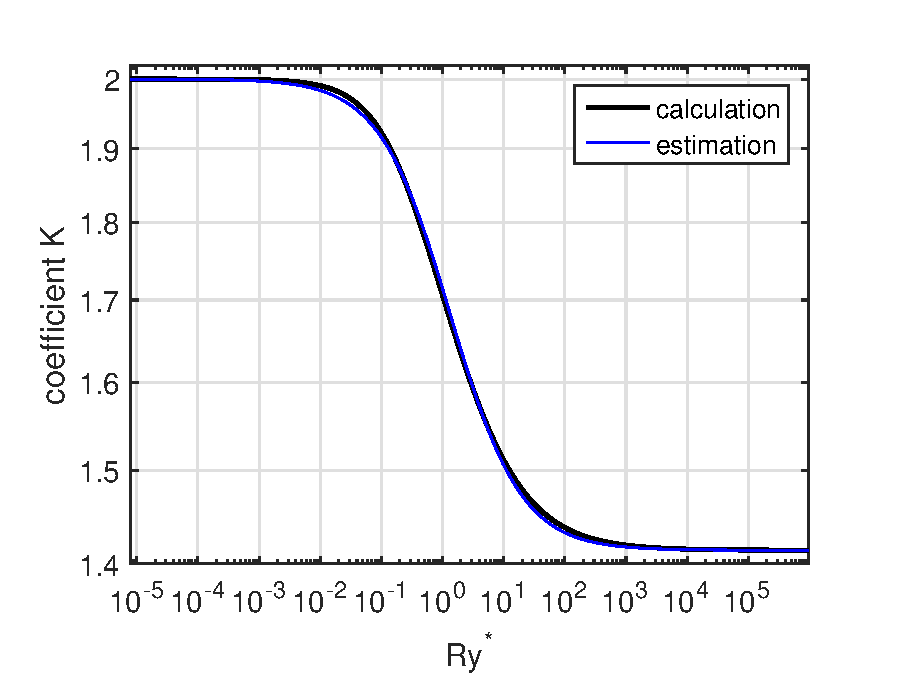
\includegraphics[width=3in]{KvR}}
						\subfloat[relative error changes with $Ry^{*}$  ]{\label{fig:EvR.KvR}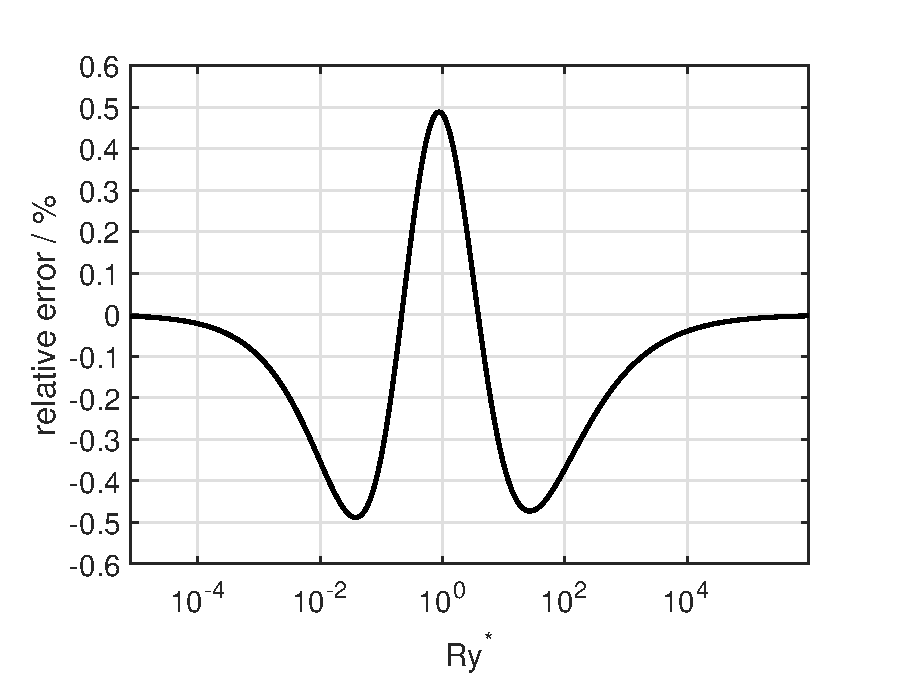
\includegraphics[width=3in]{EvR@KvR}}
					\end{center}
					\caption{Results of approximation of coefficient $K$ against $Ry^{*}$  }
					\label{fig:A.KvR}
				\end{figure*}
	\autoref{eq:Sm} can be written as a function depicting the near field temperature distribution around the maximum temperature point:
	\begin{equation} \label{eq:near field}
		Ry^{*}=Ry_{min}^{*}\left(\sigma^{*}\right)e^{\frac{y_m^{*2}}{K^2\sigma^{*2}}}
	\end{equation}
	\section{quasi point source}
		When $\sigma^{*}=0$, the  \autoref{eq:original} describes the point heat source.
		\begin{eqnarray}\label{eq:gauss v point 0}
		\frac{1}{\sqrt{2\pi}}\int_{0}^{\infty}{d\tau}\quad \tau^{-\frac{3}{2}}e^{-\frac{x^{*2}+2\tau^*x^{*}+\tau^{*2}+y^{*2}}{2\tau}} = \frac{1}{r^{*}}e^{-r^{*}-x^{*}}
		\end{eqnarray}
	Do derivations on \autoref{eq:gauss v point 0} with respect to y:
		\begin{eqnarray}\label{eq:gauss v point}
		\frac{1}{\sqrt{2\pi}}\int_{0}^{\infty}{d\tau}\quad \tau^{-\frac{3}{2}}e^{-\frac{x^{*2}+2\tau^*x^{*}+\tau^{*2}+y^{*2}}{2\tau}} = \frac{1}{r^{*}}e^{-r^{*}-x^{*}} \label{eq:gauss v point 1}
		\\
		\frac{1}{\sqrt{2\pi}}\int_{0}^{\infty}{d\tau}\quad \tau^{-\frac{5}{2}}e^{-\frac{x^{*2}+2\tau^*x^{*}+\tau^{*2}+y^{*2}}{2\tau}} = -\frac{1}{y^{*}}  \frac{\partial}{\partial y^{*}}\left(\frac{1}{r^{*}}e^{-r^{*}-x^{*}}\right)=e^{-r^{*}-x^{*}}\left(\frac{1}{r^{*2}}+\frac{1}{r^{*3}}\right)  \label{eq:gauss v point 2}
		\\
		\frac{1}{\sqrt{2\pi}}\int_{0}^{\infty}{d\tau}\quad \tau^{-\frac{7}{2}}e^{-\frac{x^{*2}+2\tau^*x^{*}+\tau^{*2}+y^{*2}}{2\tau}} =\frac{1}{y^{*}}  \left[\frac{1}{y^{*}}  \frac{\partial}{\partial y^{*}}\left(\frac{1}{r^{*}}e^{-r^{*}-x^{*}}\right)\right] =e^{-r^{*}-x^{*}}\left(\frac{1}{r^{*3}}+\frac{3}{r^{*4}} +\frac{3}{r^{*5}}\right) \label{eq:gauss v point 3}
		\end{eqnarray}
		
	When $\frac{\sigma^{*}}{\sigma^{*}_m}$ tends to zero, the Gaussian heat source can be treated as point source, with little error. So, use \autoref{eq:original} rather than \autoref{eq:gover}.
		\begin{eqnarray}  \label{eq:farfield}
			\nonumber
		T^*=\frac{1}{\sqrt{2\pi}}\int_{0}^{\infty}{d\tau}\frac{\tau^{-\frac{1}{2}}}{\tau+\sigma^{*2}}e^{-\frac{x^{*2}+2\tau^*x^{*}+\tau^{*2}+y^{*2}}{2\tau+2\sigma^{*2}}}
		\\ \nonumber
			\approx \frac{1}{\sqrt{2\pi}}\int_{0}^{\infty}{d\tau}\;{\tau^{-\frac{3}{2}}}e^{-\frac{x^{*2}+2\tau^*x^{*}+\tau^{*2}+y^{*2}}{2\tau}} \cdot \left[ \left(1+\frac{\sigma^{*2}}{2} \right)   +\sigma^{*2}\left(x-1\right)\frac{1}{\tau}   +\frac{x^{*2}+y^{*2}}{2}\sigma^{*2}\frac{1}{\tau^2}\right]
		\\ 
			= e^{-r^{*}-x^{*}}\left[ \left(1+\frac{\sigma^{*2}}{2} \right)  \frac{1}{r^{*}} +\sigma^{*2}\left(x-1\right) \left(\frac{1}{r^{*2}}+\frac{1}{r^{*3}}\right)
			 +\frac{\sigma^{*2}}{2}\left(\frac{1}{r^{*}}+\frac{3}{r^{*2}} +\frac{3}{r^{*3}}\right)\right]
		\end{eqnarray}
		This process uses the first two terms of Taylor series of integrand with respect to $\sigma^{*}$. \autoref{eq:farfield} describes the temperature distribution of far field.
	\subsection{$\sigma\rightarrow{0}$}
	When $\sigma\rightarrow{0}$, $x^{*} \ll y^{*}\ll 1$.\autoref{eq:farfield} can be simplified as
		\begin{eqnarray}  \label{eq:farfield.01}
		\nonumber
		T^*
		\approx e^{-r^{*}-x^{*}}\left[ \left(1+\frac{\sigma^{*2}}{2} \right)  \frac{1}{r^{*}} +\sigma^{*2}\left(x-1\right) \left(\frac{1}{r^{*2}}+\frac{1}{r^{*3}}\right)
		+\frac{\sigma^{*2}}{2}\left(\frac{1}{r^{*}}+\frac{3}{r^{*2}} +\frac{3}{r^{*3}}\right)\right]
		\\ \nonumber
		\approx 1\cdot \left[ \left(1+\frac{\sigma^{*2}}{2} \right)  \frac{1}{y^{*}}-\sigma^{*2}\frac{1}{y^{*3}}
		+\frac{\sigma^{*2}}{2}\frac{3}{y^{*3}}\right]
		\\ \nonumber
		\approx  \frac{1}{y^{*}}+\frac{\sigma^{*2}}{2}\frac{1}{y^{*3}}
		\end{eqnarray} 
		Use perturbation method, $y^*_{m,gauss}=y^*_{m,point}\left(1+a\sigma^{*2}\right)$, $a\sigma^{*2}\ll1$ ,	$y^*_{m,point}=Ry^{*}$.
		\begin{eqnarray}  
		\nonumber
		\frac{1}{Ry^{*}} \approx  \frac{1}{y^{*}}+\frac{\sigma^{*2}}{2}\frac{1}{y^{*3}}
		\approx\frac{1}{y^*_{m,point}\left(1+a\sigma^{*2}\right)}+\frac{\sigma^{*2}}{2}\frac{1}{y^{*3}_{m,point}\left(1+3a\sigma^{*2}\right)}
		\\ \nonumber 
		\approx \frac{1}{Ry^{*}\left(1+a\sigma^{*2}\right)}+\frac{\sigma^{*2}}{2}\frac{1}{Ry^{*3}\left(1+3a\sigma^{*2}\right)}
		\\
		\Rightarrow a=\frac{1}{2Ry^{*2}}  \label{eq:farfield.0.a}
		\\
		y^*_{m,gauss,0}=y^{*}_{m,point}\left(1+\frac{1}{2Ry^{*2}}\sigma^{*2}\right)\label{eq:farfield.0}
		\end{eqnarray} 
		
	\subsection{$\sigma\rightarrow{\infty}$}
	When $\sigma\rightarrow{\infty}$, $1 \ll \sigma^{*}\ll y^{*} \ll x^{*}$.\autoref{eq:farfield} can be simplified as
	\begin{eqnarray}  \label{eq:farfield.inf.1}
	\nonumber
	T^*
	\approx e^{-r^{*}-x^{*}}\left[ \left(1+\frac{\sigma^{*2}}{2} \right)  \frac{1}{r^{*}} +\sigma^{*2}\left(x-1\right) \left(\frac{1}{r^{*2}}+\frac{1}{r^{*3}}\right)
	+\frac{\sigma^{*2}}{2}\left(\frac{1}{r^{*}}+\frac{3}{r^{*2}} +\frac{3}{r^{*3}}\right)\right]
	\\ \nonumber
	\approx e^{-r^{*}-x^{*}}  \left[\frac{1}{r^{*}}+\frac{\sigma^{*2}\left(r^{*}+x^{*2}\right)}{r^{*2}}-\frac{\sigma^{*2}}{2r^{*2}}\right]
	\\ 
	\approx e^{\frac{1}{2}\frac{y^{*2}}{x^{*}}}  \left[-\frac{1}{x^{*}}+\frac{\sigma^{*2}}{x^{*2}}\left(-\frac{y^{*2}}{2x^{*}}-0.5\right)\right]
	\end{eqnarray} 
	Use perturbation method, $y^*_{m,gauss}=y^*_{m,point}\left(1+b\sigma^{*2}\right)$, $x^*_{m,gauss}=x^*_{m,point}\left(1+c\sigma^{*2}\right)$ , $b\sigma^{*2}\ll1$ ,$c\sigma^{*2}\ll1$, $y^*_{m,point}=\sqrt{\frac{2}{e}Ry^{*}}$,$x^*_{m,point}=-\frac{Ry^{*}}{e}$.
	\begin{eqnarray}  
		\nonumber
		\frac{1}{Ry^{*}} \approx e^{\frac{1}{2}\frac{y^{*2}}{x^{*}}}  \left[-\frac{1}{x^{*}}+\frac{\sigma^{*2}}{x^{*2}}\left(-\frac{y^{*2}}{2x^{*}}-0.5\right)\right]
		\\ \nonumber 
		\approx e^{\frac{1}{2}\frac{y^{*2}}{x^{*}}}  \left[-\frac{1}{x^{*}}+\frac{\sigma^{*2}}{x^{*2}}\left(0.5+2b\sigma^{*2}-c\sigma^{*2}\right)\right]
		\\ \nonumber
		\approx e^{\frac{1}{2}\frac{y^{*2}}{x^{*}}}  \left(-\frac{1}{x^{*}}+0.5\frac{\sigma^{*2}}{x^{*2}}\right)
		\\ \nonumber
		y^*=\sqrt{2x^*\ln{\frac{x^{*2}/Ry^{*}}{-x^{*}+0.5\sigma^{*2}}}}
		\\ \nonumber
		\frac{dy^*}{dx^*}= \dfrac{\sqrt{2}\left(2\ln\left(-\frac{2tx^2}{-s^2+2x}\right)+\frac{4x-4s^2}{-s^2+2x}\right)}{4\sqrt{x\ln\left(-\frac{2tx^2}{2x-s^2}\right)}}=0
		\\ \nonumber
		\Rightarrow x^*_{m,gauss}=x^*_{m,point}
		\\ \nonumber
		\Rightarrow b=\frac{e}{4Ry^{*}} 
		\\
		 y^{*}_{m,gauss,infinity}=y^{*}_{m,point}\left(1+\frac{e}{4Ry^{*}}\sigma^{*2}\right)
		 \label{eq:farfield.inf}
    \end{eqnarray} 
	\subsection{blending}
	Use the following equation to blending:
	\begin{equation} \label{eq:blending s/s}
		y^{*}_{m,gauss}=y^{*}_{m,point}\left(1+P*\sigma^{*2}\right)
	\end{equation}
	
	\begin{equation}
		P=\left[\left( \frac{1}{2Ry^{*2}}\right)^n+  \left( \frac{e}{4Ry^{*}}\right)^n  \right]^{\frac{1}{n}}
	\end{equation}
	Where $n=0.8655$, maximum error reaches $1.45\%$.
		\begin{figure*}[ht!]
			\begin{center}
				\subfloat[coefficient changes with $Ry^{*}$] {\label{fig:PvR}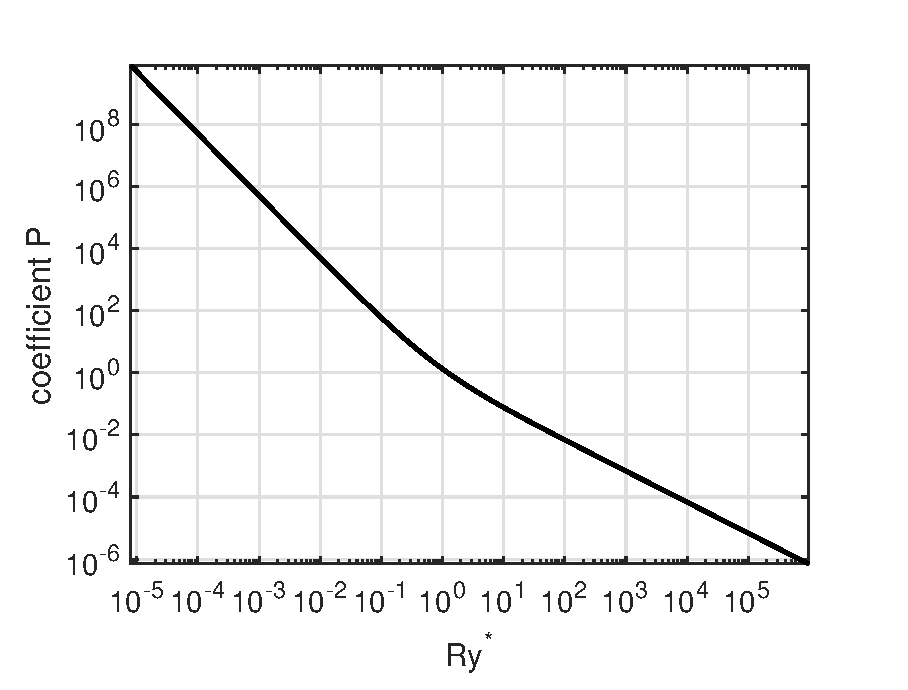
\includegraphics[width=2.2in]{PvR}}
				\subfloat[relative error changes with $Ry^{*}$  ]{\label{fig:EvR.PvR}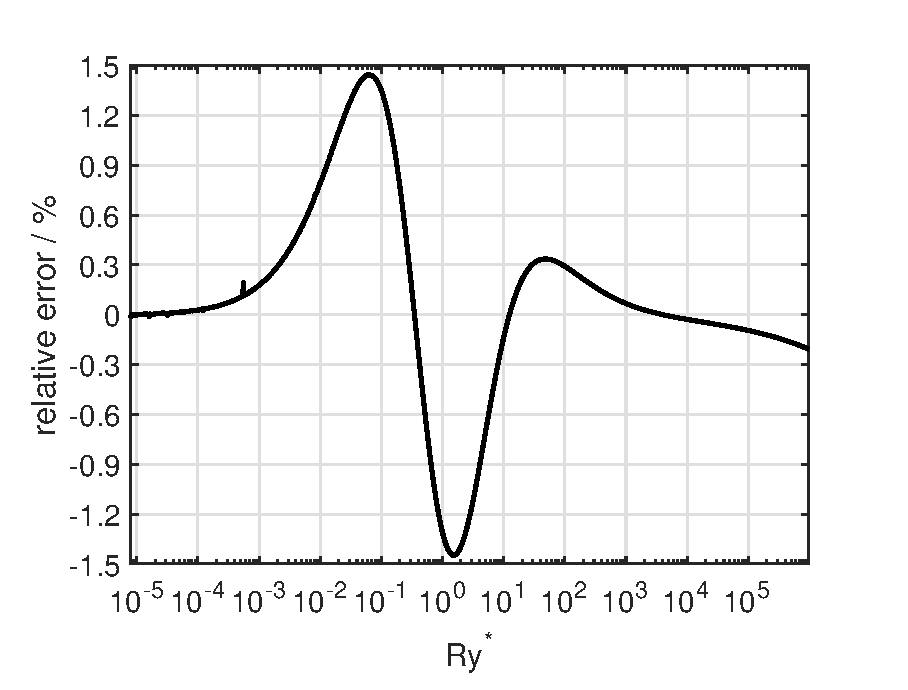
\includegraphics[width=2.2in]{EvR@PvR}}
				\subfloat[relative error changes with $Ry^{*}$  ]{\label{fig:Evn.PvR}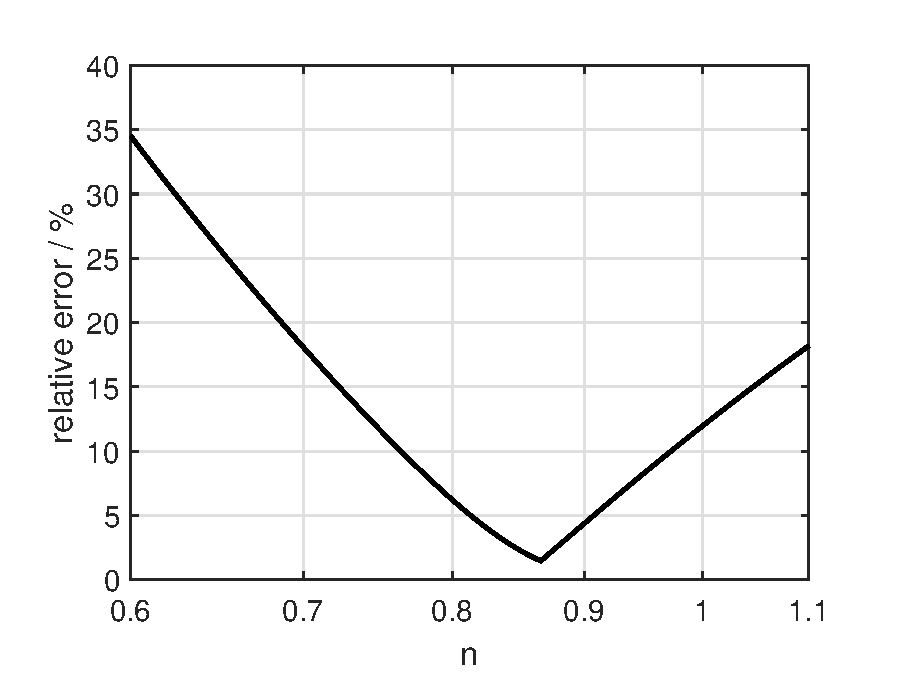
\includegraphics[width=2.2in]{Evn@PvR}}
			\end{center}
			\caption{Results of approximation of coefficient $K$ against $Ry^{*}$  }
			\label{fig:A.PvR}
			
			% 修改图
			%解释为什么后面误差不等于0; 并且举例子
		\end{figure*}
	\section{Combination}
	The maximum width of welding pool is a combination of far-field and near-field. To cover the middle range of $\frac{\sigma}{\sigma_m}$, the correction of near-field equation is needed.
	\begin{equation}  \label{eq:LvR}
    L=	0.93175-0.06825\tanh\left({-0.6571 \; \ln\dfrac{Ry}{15.926}}\right)-0.0132\sin\left[3{\pi}\tanh\left(0.2485 \; Ry^{0.3718}\right)\right]
	\end{equation}
	
		\begin{figure*}[ht!]
			\begin{center}
				\subfloat[coefficient changes with $Ry^{*}$] {\label{fig:LvR}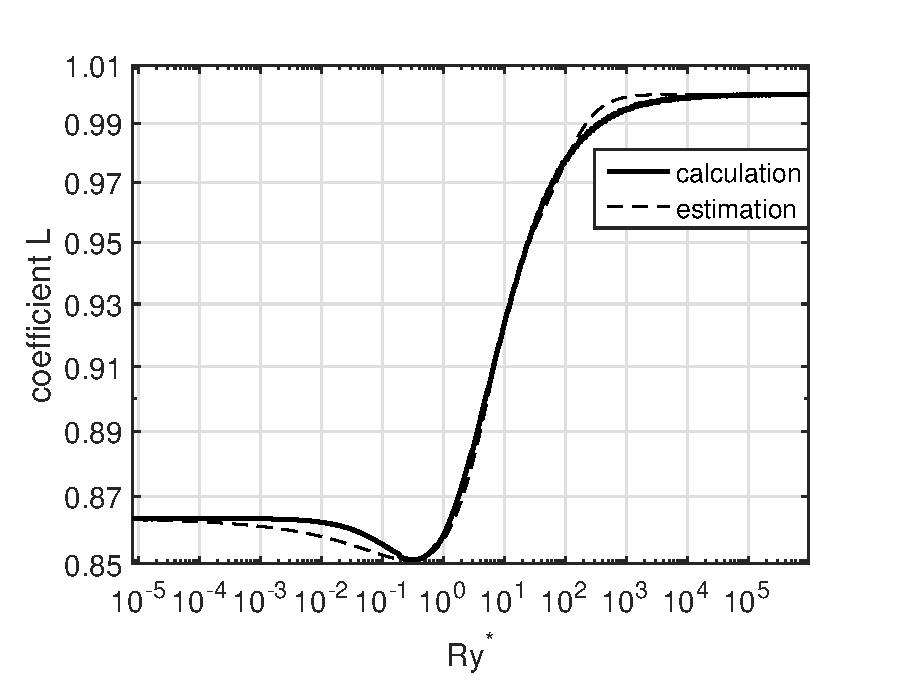
\includegraphics[width=2.2in]{LvR}}
				\subfloat[relative error changes with $Ry^{*}$  ]{\label{fig:E.LvR}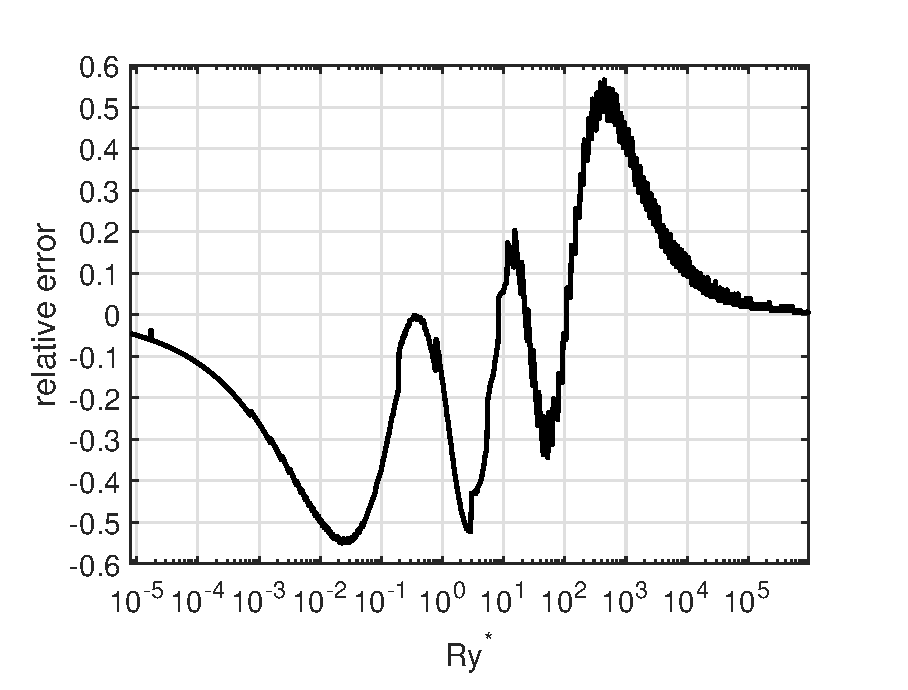
\includegraphics[width=2.2in]{E@LvR}}
			\end{center}
			\caption{Results of approximation of coefficient $L$ against $Ry^{*}$  }
			\label{fig:A.LvR}
		\end{figure*}
   The maximum error reaches $0.55\%$. 
   
   
   
	\section{whole plane}
		\begin{align}  
		y_m^*\;  & =  MAX\{ \quad y_{m,1}^* \; , \quad  y_{m,2}^* \quad \}
			\\\nonumber
		y_{m,1}^*& =\left\{
				\begin{aligned}
					& y_{m,point}^*\left(1+P\sigma^{*2}\right)  \qquad 
					      &\frac{\sigma^*}{\sigma^*_m}   <    \;    lin\\
				    & 0   &\frac{\sigma^*}{\sigma^*_m}   \geq \;    lin
				\end{aligned}
				\right.
			\\ \nonumber
		y_{m,2}^*& = K\left[L\left(\sigma^*-\sigma^{*}_m\right)+\sigma^{*}_m 	\right]\sqrt{\ln{\frac{Ry^{*}}{Ry_{min}^{*}(\sigma^{*})}}}
		\end{align} 
		The parameters in equations are as follows:
		\begin{align}
		\nonumber
			y_{m,point}^* &=\left[\left(Ry^*\right)^n+  \left( \sqrt{\frac{2}{e}Ry^{*}}\right)^n  \right]^{\frac{1}{n}}    
			\\ \nonumber &\quad \quad \mbox{\mbox{Where}  \quad  n= \; -1.7312}
			\\ \nonumber
			P \quad      & =\left[\left( \frac{1}{2Ry^{*2}}\right)^n+  \left( \frac{e}{4Ry^{*}}\right)^n  \right]^{\frac{1}{n}}    
			\\ \nonumber &\quad \quad \mbox{\mbox{Where}  \quad  n= \; 0.8655}
			\\  \nonumber 
			lin \quad      & =0.1\left(Ry^*>5\times10^3\right)+0.4\left(Ry\leqslant5\times10^3\right);   
			\\ \nonumber
			K \quad      &=k_0-A*\tanh{\left(B\ln{\frac{Ry}{C}}\right)}
			\\ \nonumber & \quad \quad \mbox{Where $k_0=\frac{2+\sqrt{2}}{2}$,$A=\frac{2-\sqrt{2}}{2}$,$B=0.3775$,$C=1.0690$.} 
			\\ \nonumber
			L \quad     &= 
			0.93175-0.06825\tanh\left({-0.6571 \; \ln\dfrac{Ry}{15.926}}\right)-0.0132\sin\left[3{\pi}\tanh\left(0.2485 \; Ry^{0.3718}\right)\right]
			\\ \nonumber
			\sigma^{*}_{m}\quad & =\left[ \left( 1.0140 \; Ry^{*\frac{2}{3}}\right)^n+ \left( \sqrt{\frac{\pi}{2}}Ry^{*}\right)^n\right]^\frac{1}{n}
			\\ \nonumber & \quad \quad\mbox{Where $n=-2.3975$}				
			\\ \nonumber
			Ry_{min}^{*}(\sigma^{*})& = \left[ \left( \sqrt{\frac{\pi}{2}}    \; \sigma^{*-1}\right)^n+ \left(\frac{2.5596}{\sqrt{2\pi}} \; \sigma^{*-1.5}\right)^n\right]^{-\frac{1}{n}}	
			\\ \nonumber
				       & \quad \quad \mbox{Where $n=-1.9464$}
		\end{align}
		The maximum error reaches $5.25\%$.There is a limit that $\frac{\sigma^*}{\sigma_m^*}<98\%$, because when $\frac{\sigma^*}{\sigma_m^*}$ tends to $1$, $y_m^*$ tends to $0$,  the approximation (means that it's not accurate) of $Ry_{min}^* , \sigma_m^*$ leads to a large relative error. If the high-precision value is obtained, these equations still work.
		\begin{figure}
				\centering	
				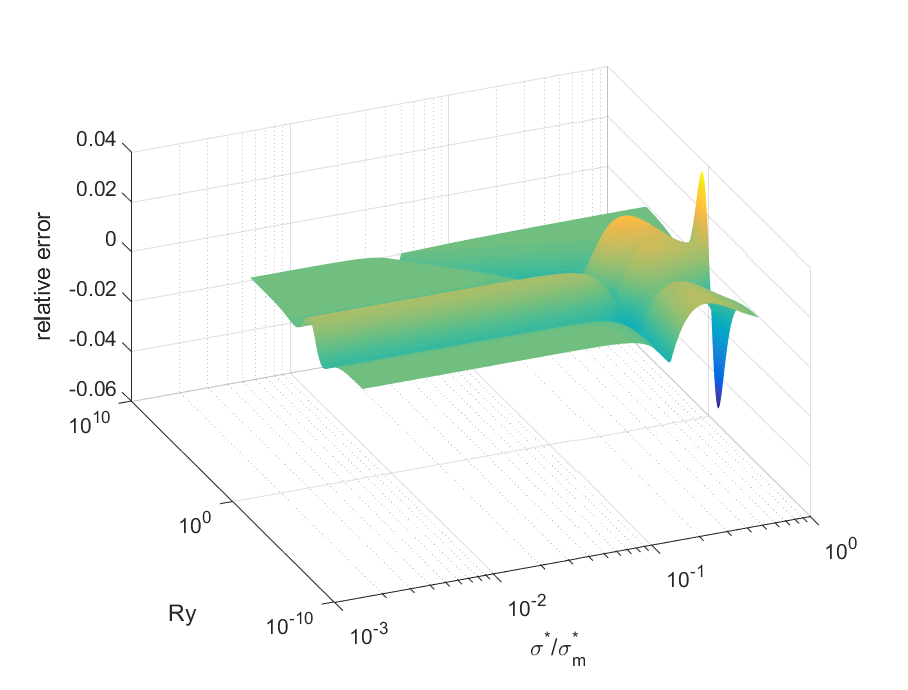
\includegraphics[width=4in]{all_E.eps}
				\caption{relative error over whole plane.}	
				\label{fig:all_E}
		\end{figure}
	%%%%%%%%%%%%%%%%%%%%%%%%%%%%%%%%%%%%%%%%%%%%%%%%%%
	%%%              RESULTS SECTION              %%%%
	%%%%%%%%%%%%%%%%%%%%%%%%%%%%%%%%%%%%%%%%%%%%%%%%%%		    
	\section{Results}\label{sec:results}
	Results
	%%%%%%%%%%%%%%%%%%%%%%%%%%%%%%%%%%%%%%%%%%%%%%%%%%
	%%%              DISCUSSION SECTION              %%%%
	%%%%%%%%%%%%%%%%%%%%%%%%%%%%%%%%%%%%%%%%%%%%%%%%%%		      
	\section{Discussion}\label{sec:discussion}
	

	%\begin{itemize}
	%	\item nitrogen can be used to limit the amount of G-phase, but not eliminate it all together. This may not alleviate the liquation cracking problems. There is also the question of what Z-phase and potentially $\pi$-phase would do to the alloy, negative or positive. Can only relate to microstructure analyzed by Danielson for clues.
	%	\item carbon influence on $\rm M_{23}C_{6}$
	%	\item $\pi$-phase precipitates at the expense of Z-phase. Increased Si will promote $\pi$-phase. Nb promotes Z-phase or G-phase at expense of $\pi$-phase.
	%	\item high carbon and nitrogen content forces high stability temperature for $\rm M_{23}C_{6}$ because of Nb/(C+N) ratio.
	%\end{itemize}
	
	%%%%%%%%%%%%%%%%%%%%%%%%%%%%%%%%%%%%%%%%%%%%%%%%%%
	%%%              CONCLUSIONS SECTION              %%%%
	%%%%%%%%%%%%%%%%%%%%%%%%%%%%%%%%%%%%%%%%%%%%%%%%%%		
	
	\section{Conclusions}
	\indent Conclusions Section
	

%\begin{itemize}
%	\item nitrogen can be used to limit the amount of G-phase, but not eliminate it all together. This may not alleviate the liquation cracking problems. There is also the question of what Z-phase and potentially $\pi$-phase would do to the alloy, negative or positive. Can only relate to microstructure analyzed by Danielson for clues.
%	\item carbon influence on $\rm M_{23}C_{6}$
%	\item $\pi$-phase precipitates at the expense of Z-phase. Increased Si will promote $\pi$-phase. Nb promotes Z-phase or G-phase at expense of $\pi$-phase.
%	\item high carbon and nitrogen content forces high stability temperature for $\rm M_{23}C_{6}$ because of Nb/(C+N) ratio.
%\end{itemize}
	      
%%%%%%%%%%%%%%%%%%%%%%%%%%%%%%%%%%%%%%%%%%%%%%%%%%
%%%              CONCLUSIONS SECTION              %%%%
%%%%%%%%%%%%%%%%%%%%%%%%%%%%%%%%%%%%%%%%%%%%%%%%%%		

	\section{Conclusions}
	\indent Conclusions Section

%%%%%%%%%%%%%%%%%%%%%%%%%%%%%%%%%%%%%%%%%%%%%%%%%%
%%%              Acknowledgement SECTION              %%%%
%%%%%%%%%%%%%%%%%%%%%%%%%%%%%%%%%%%%%%%%%%%%%%%%%%	
	\section{Acknowledgement}
	\indent This study has been supported by...      			
	
\section{References}
\bibliography{References/references}   % .bib info
%%%%%%%%%%%%%%%%% Reference Style %%%%%%%%%%%%%%%%%%%
% Needs to be changed based on the journal you are sumbitting to. 
% see ``bst\journal_refstyles.pdf'' for more information
\bibliographystyle{bst/model3-num-names}		
2
\end{document}